\chapter{Analysis of high-temperature events}

\label{Chapter5}

In this chapter, the products of HTE monitoring from MITIP will presented firstly using several scenes worldwide which contains volcanoes, large scale lava flow and wild fires. In section 5.2, the HTE monitoring results of MITIP will be compared with the results of the Zhukov's algorithm, which is used to process the TET-1 imagery in the receive center.\\
%----------------------------------------------------------------------------------------
%	SECTION 1
%----------------------------------------------------------------------------------------

\section{High-temperature events}
In this section, the HTE monitoring results are presented. For the processing of all scenes, the maps of MODIS water vapor, ASTER DEM and 8.6 $\mu$m emissivity were provided and resampled to the TET-1 imagery's size and pixel size. The input TET-1 MIR and TIR TOA radiance values are scaled with scale factor 1.15 and 1.05 respectively.\\

%-----------------------------------
%	SUBSECTION 1
%-----------------------------------

\subsection{Volcanoes}
First of all, the HTE monitoring products of Etna and Stromboli in the date 2016.06.22 are presented. Both of them only occupy a little spaces in images because of their small sizes.

\begin{figure}[!htbp]
\centering
\subfigure[MIR band]{
\label{fig:Etna_mir_tem}
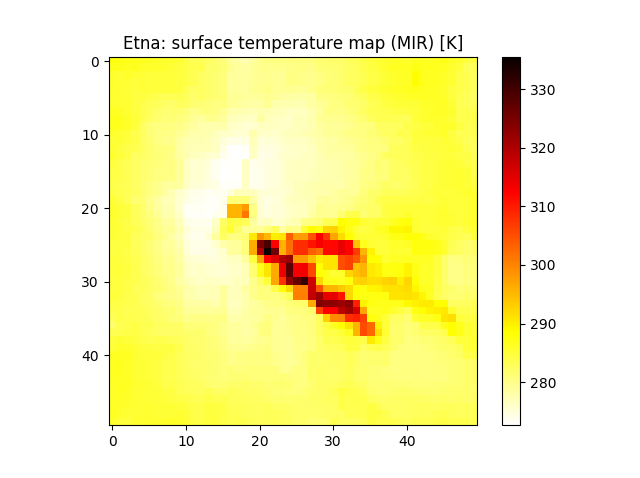
\includegraphics[width = 0.8\linewidth]{temp_map_etna_mir.png}}
\hspace{0.1in}
\subfigure[TIR band]{
\label{fig:Etna_tir_tem}
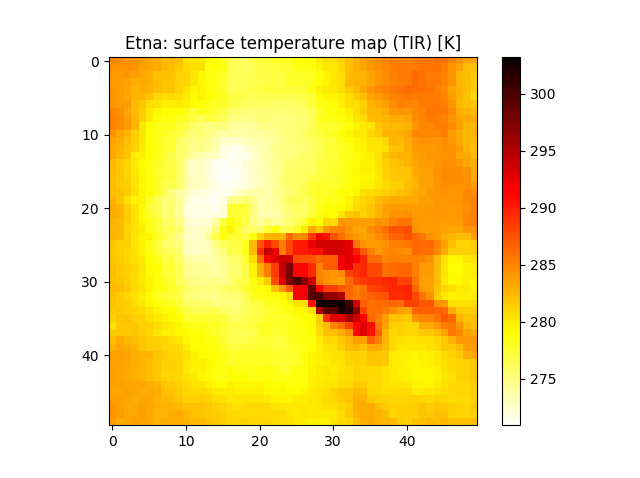
\includegraphics[width = 0.8\linewidth]{temp_map_etna_tir.png}}
\caption{Surface temperature maps of Etna 2014.06.22.}
\label{fig:Etna_sur_tem}
\end{figure}

\noindent As Figure \ref{fig:Etna_sur_tem} shows, the surface temperatures of the lava are around 310 K to 340K in MIR band and 290K to 310K in TIR band. The effective target temperature in sub-pixel resolution and effective target pixel fraction as well as the FRP are shown in Figure \ref{fig:Etna_HTE}. We can see that no all hot pixels in the surface temperature maps are solved for the effective target temperature and target pixel fraction due to numerical reasons. The hottest areas of the Etna is around 850 K. It can be notice that the higher the effective target temperature in one pixel, the lower the effective target pixel fraction of it because the pixel temperature and background temperature are pre-determined.\\

\begin{figure}[!htbp]
\centering
\subfigure[Effective target temperature]{
\label{fig:Etna_eff_tem}
\includegraphics[width = 0.65\linewidth]{Effective_target_tem2.png}}
\subfigure[Effective target pixel fraction]{
\label{fig:Etna_eff_fra}
\includegraphics[width = 0.65\linewidth]{Effective_target_pixel_frac2.png}}
\hspace{0.1in}
\subfigure[FRP]{
\label{fig:Etna_frp}
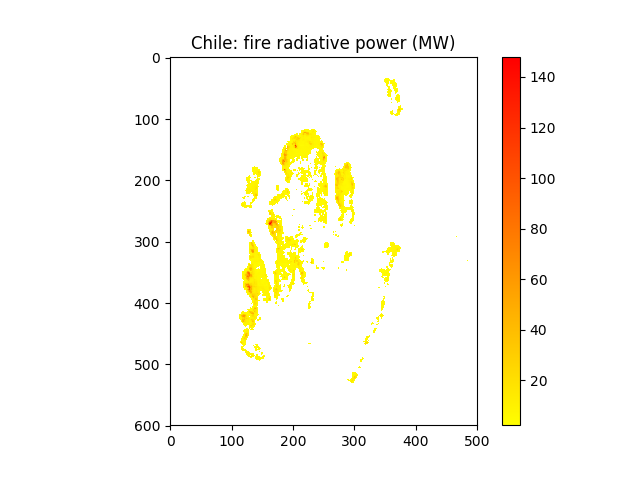
\includegraphics[width = 0.65\linewidth]{frp.png}}
\caption{HTE monitoring products of Etna 2014.06.22.}
\label{fig:Etna_HTE}
\end{figure}



%-----------------------------------
%	SUBSECTION 2
%-----------------------------------

\subsection{Fire events}

%----------------------------------------------------------------------------------------
%	SECTION 2
%----------------------------------------------------------------------------------------

\section{Comparison with the results of the Zhukov's algorithm}

%-----------------------------------
%	SUBSECTION 1
%-----------------------------------

\subsection{Brief description of Zhukov's algorithm}

%-----------------------------------
%	SUBSECTION 2
%-----------------------------------

\subsection{From pixel-based to cluster-based analysis}

%-----------------------------------
%	SUBSECTION 3
%-----------------------------------

\subsection{Comparision}

%----------------------------------------------------------------------------------------
%	SECTION 3
%----------------------------------------------------------------------------------------

% \section{Bardarbunga}

%----------------------------------------------------------------------------------------
%	SECTION 4
%----------------------------------------------------------------------------------------

% \section{Chile}

%----------------------------------------------------------------------------------------
%	SECTION 5
%----------------------------------------------------------------------------------------

% \section{Portugal}